% -*- mode: latex; mode: auto-fill; coding: utf-8; -*-

The main advantage of representing an implicit contour or surface as
a signed distance field (SDF), is that the length of the gradient is
1. This is also exactly what defines a signed distance field.

When constructing or manipulating a SDF defined on a Cartesian grid,
the result is not always a SDF. So to enable further calculations or
iterations of an algorithm the result must be turned into a new SDF
that reflects the changes done by the calculations. This process is
called \dit{reinitialization} of the implicit function, and can be
done several different ways.

Algorithms to reinitializing SDFs focus on reinitializing the whole
domain, and at the same time keeping the zero level set as fixed as
possible. This means that the process disrupts data outside the zero
level set, which depending on the type of phenomena being modeled
can be problematic. For the problems we are modelling this is not an
issue and is therefore not of relevance here.

Before diving into the algorithms a good question is, how often must the
implicit function be reinitialized? There is no good answer to this
question, because it depends on how rapidly the contour is
changing. In our work we have been reinitializing after every change,
which ensures that this is not a source of error.

The two most used algorithmic approaches to reinitialization are:
methods that geometrically calculate distances to the contour or surface,
and PDE based methods that numerically approximate solutions to the
Eikonal equation: $||\nabla \phi|| = 1$
\citbook{bridson2008fluid}{page~89}.

When initializing the implicit contour in section \vref{sec:initialization}
we used an algorithm that geometrically calculated the distance to the
contour. So the natural choice would have been also to use this algorithm for
reinitializing, but because the algorithm does not calculate the
SDF precise enough, we cannot use the algorithm
when reinitializing. Furthermore if we had used this type of
algorithm, we would have had to construct the contour before
invoking the algorithm. Constructing the contour is very expensive,
and is something that should be avoided at almost all cost when using
the level set method. Instead we have chosen to use PDEs to solve the
Eikonal equation.

\subsection{The PDE way of reinitializing}
When using the PDE way of reinitializing the level set, we solve the
following PDE \citbook{osher2002level}{page~65-66}:

\begin{equation}
\label{eq:reinit}
\phi_t + S(\phi_0)(|\nabla \phi| - 1) = 0
\end{equation}

Where $\phi$ is the SDF being evolved as a PDE, and $\phi_0$, is the
initial SDF given as input to the reinitialization algorithm, which
has not been altered by the process of solving the PDE. The function
$S(\phi_0)$ gives the sign of the SDF, like the following function,
described in \citbook{osher2002level}{page~66}:
%\citbook{article:FLLSM}{page~419}:

\begin{equation}
\label{eq:s1}
S(\phi) =
\begin{cases}
-1 &\mbox{ if } \phi < 0, \\
 0 &\mbox{ if } \phi = 0, \\
 1 &\mbox{ if } \phi > 0.
\end{cases}
\end{equation}

When using this approach of reinitializing the SDF, the grid
points in $\phi$ that are nearest to the contour is reinitialized
first, and then propagated in the normal direction from the zero
level set, hereby reinitializing the grid points in layers around the
zero level set, reinitializing a new layer each iteration.

This algorithm is relatively slow if all grid points need to be
reinitialized, because it only reinitializes one layer in each
iteration when solving the PDE. This means that the PDE, on a
two-dimensional domain, must be iterated
$\sqrt{width^2 \times height^2}$ times to make sure that the algorithm
has reinitialized the whole domain. \todoCpvc{we do this only 30 times}

But because the algorithm has the property of reinitializing the SDF
in layers it is of special interest in regards to performance when
using a narrow band level set as described in section
\vref{sec:narrowband}. Here only three or four layers around the SDF needs
to be reinitialized, making the algorithm ideal for the narrow band
approach.

\subsection{The sign function S}
Because equation \ref{eq:reinit} is a hyperbolic PDE, we need to use a
smeared out version of equation \eqref{eq:s1}. One way of smearing the
function is to use equation \eqref{eq:Sphi0}.

\begin{equation}
\label{eq:Sphi0}
S(\phi_0) = \frac{\phi_0}{\sqrt{\phi_0^2 + (\Delta x)^2}}
\end{equation}

The difference between equation \eqref{eq:s1} and equation
\eqref{eq:Sphi0} can more easily be seen by looking at plots of the
two functions, as depicted in figure \ref{fig:s-graph}.

\begin{figure}[h]
\begin{center}
  \subfloat[Plot of equation \eqref{eq:s1}]{
    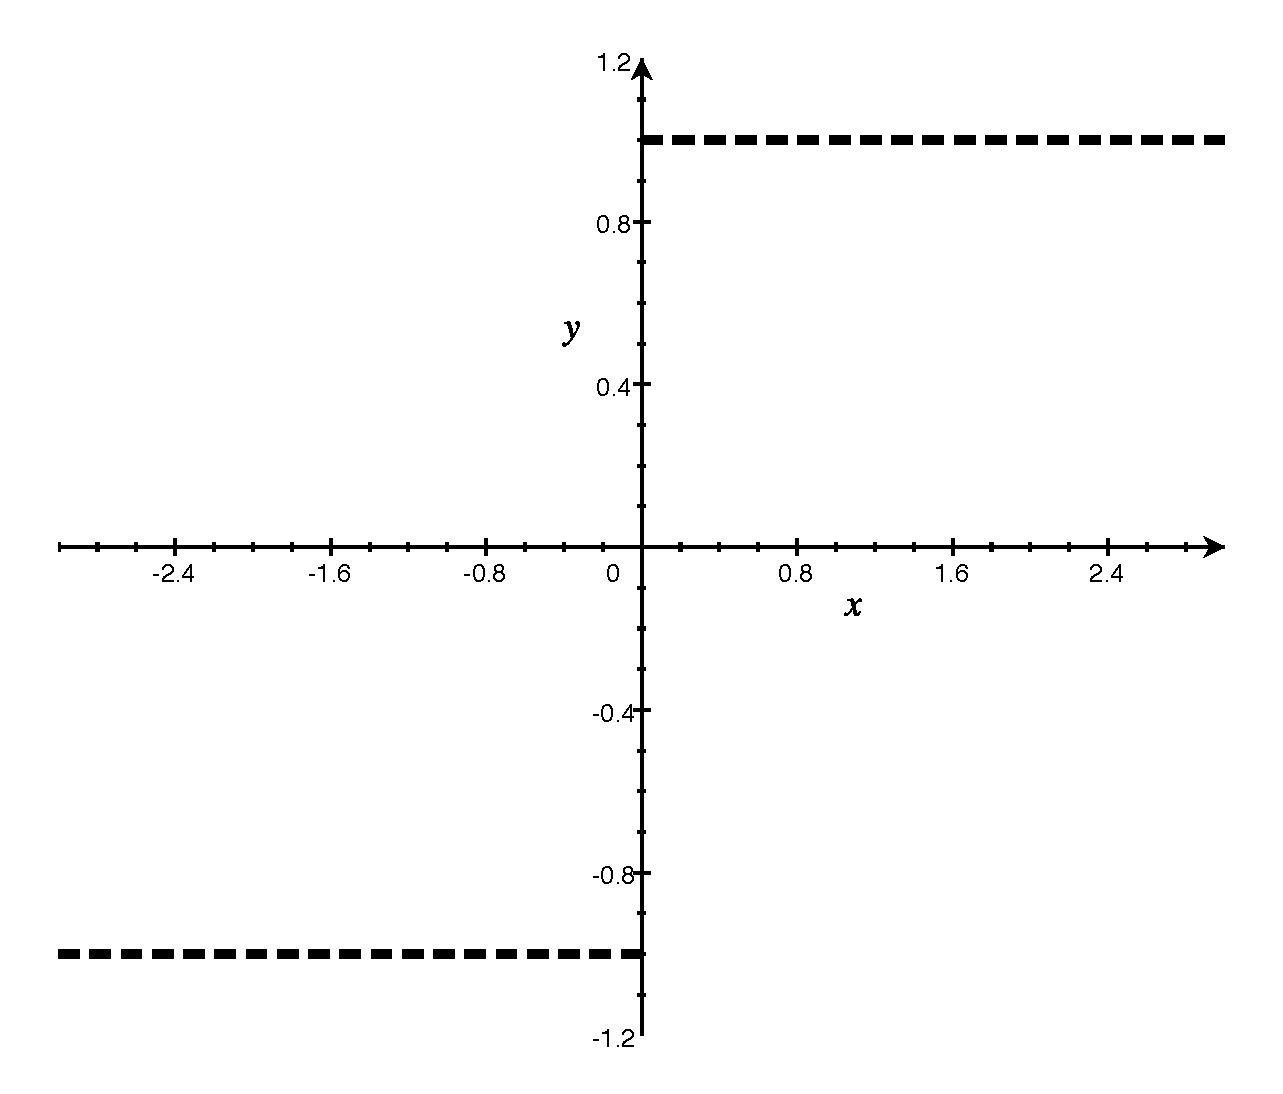
\includegraphics[width=0.5\textwidth]{imgs/S0.pdf}
    \label{fig:fake1}
  }
  \subfloat[Plot of equation \eqref{eq:Sphi0}, $\Delta x=1$]{
    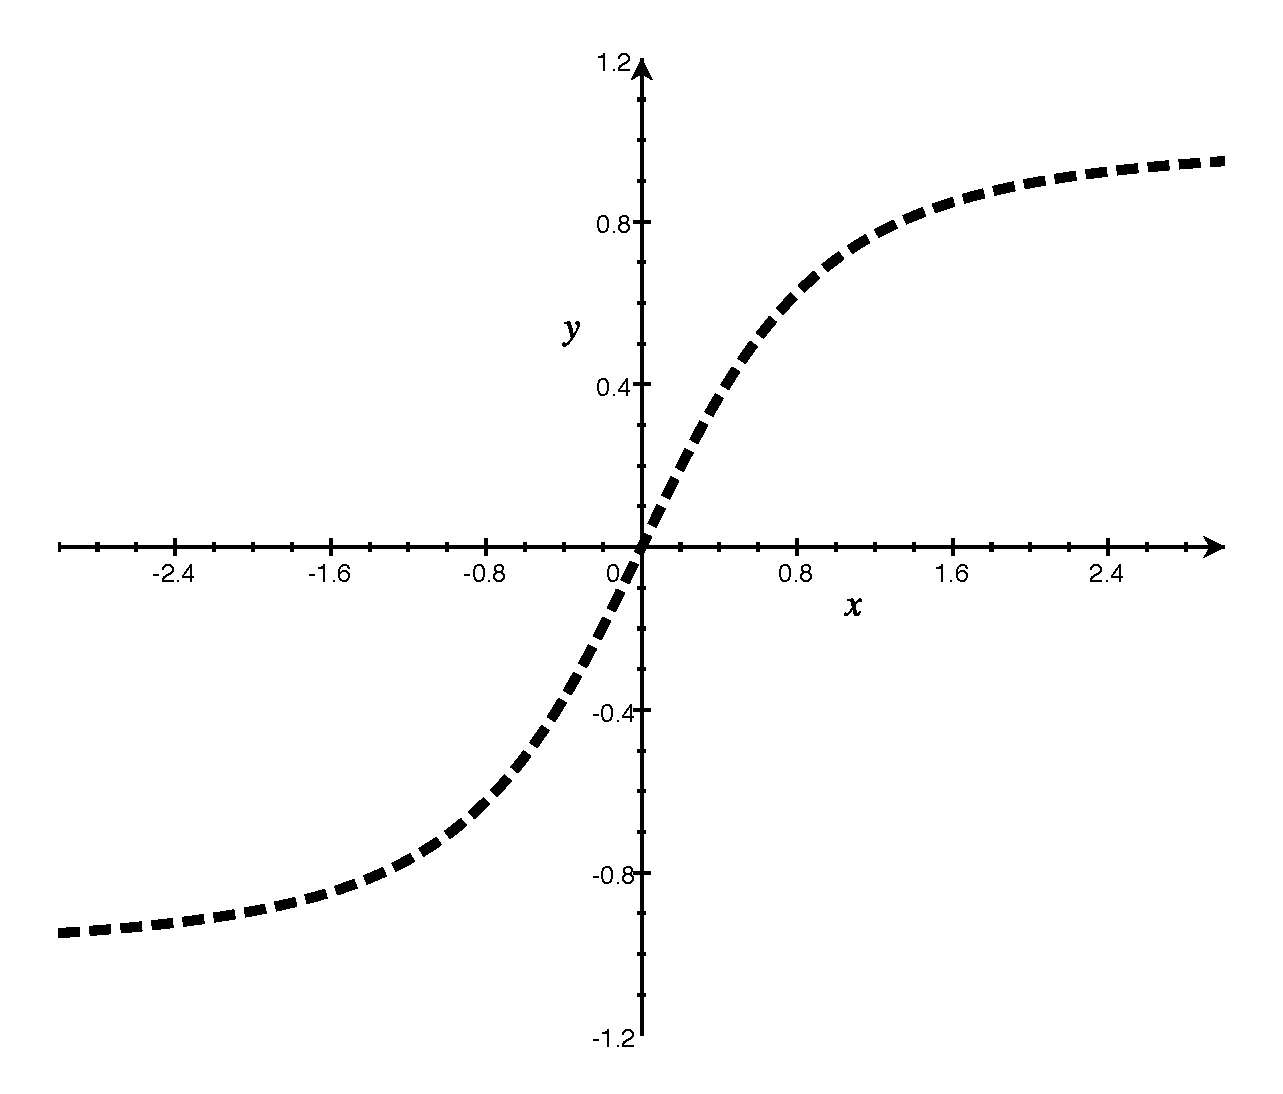
\includegraphics[width=0.5\textwidth]{imgs/S1.pdf}
    \label{fig:fake2}
  }
\end{center}
\caption{Illustrations of S}
\label{fig:s-graph}
\end{figure}

%\subsection{CFL-condition}


\pagebreak
\subsection{Implementation}
The implementation of how to solve the PDE in equation \eqref{eq:reinit},
uses the description of Godunov's scheme from
\citbook{osher2002level}{page~58} in the spatial dimensions, and a
forward Euler in the temporal dimension, as described in formula
(1.3) in \citbook{osher2002level}{page~10}.

\begin{lstlisting}[language=c++]
    Tex<float> phi0 = GetPhi(); Tex<float> phin = GetPhi();
    for (unsigned int i = 0; i<iterations; i++) {
        for (unsigned int x = 0; x < width; x++) {
            for (unsigned int y = 0; y < height; y++) {
                float xy = phi(x, y);                
                float phiXPlus = 0.0f;
                float phiXMinus = 0.0f;
                float phiYPlus = 0.0f;
                float phiYMinus = 0.0f;        	
                if (x != width-1) phiXPlus  = (phi(x+1, y) - xy);
                if (x != 0)       phiXMinus = (xy - phi(x-1, y));
                if (y !=height-1) phiYPlus  = (phi(x, y+1) - xy);
                if (y != 0)       phiYMinus = (xy - phi(x, y-1));
        	
                float dXSquared = 0;
                float dYSquared = 0;
                float a = phi0(x,y);
                if (a > 0) {
                    // formula 6.3 page 58
                    float max = std::max(phiXMinus, 0.0f);
                    float min = std::min(phiXPlus, 0.0f);
                    dXSquared = std::max(max*max, min*min);
                    max = std::max(phiYMinus, 0.0f);
                    min = std::min(phiYPlus, 0.0f);
                    dYSquared = std::max(max*max, min*min);
                } else {
                    // formula 6.4 page 58
                    float max = std::max(phiXPlus, 0.0f);
                    float min = std::min(phiXMinus, 0.0f);
                    dXSquared = std::max(max*max, min*min);
                    max = std::max(phiYPlus, 0.0f);
                    min = std::min(phiYMinus, 0.0f);
                    dYSquared = std::max(max*max, min*min);        				
                }
                float normSquared = dXSquared + dYSquared;           
                float norm = sqrt(normSquared);

                // Using the S(phi) sign formula 7.6 on page 67
                float sign = phi0(x,y) / sqrt(phi0(x,y)*phi0(x,y) + 1);
                float dt = 0.3; // A stabil CFL condition
                phin(x,y) = phi(x,y) - sign*(norm - 1)*dt;
            }
        }
        for (unsigned int y=0; y<height ; y++)
            for (unsigned int x=0; x<width; x++)
                phi(x,y) = phin(x,y);

    }
\end{lstlisting}

%%% Local Variables: 
%%% mode: latex
%%% TeX-master: "../master.tex"
%%% End: 
